\documentclass[../TFG_Report.tex]{subfiles}
 
\begin{document}



\subsection{Airfoil selection}

In this section, the selection of the airfoils for the blades will be made. First, the desired characteristics will be defined. The low Reynolds influence will be described, and a study methodology will be chosen according to it. Then, several existing airfoils will be selected to be studied and a selection criteria will be detailed.Finally, the elected airfoil will be characterized. 


\subsubsection{Desired characteristics}

The desired performance of the blades varies from root to tip. The optimal solution would be to have blades with aerodynamic twist and adapt the airfoil selection to the different circumstances of each section of the blade. However, this would difficult the optimization of the chord and geometric twist distribution, so only one airfoil will be selected. \\

This selection is a compromise between aerodynamic and structural issues. Usually, a high relative thickness is used at the root (around 35\%) and a lower one at the tip (18\%). The biggest drawback of a single-airfoil blade is that this could not be done. The desired characteristics of the airfoil are enumerated in the following list: \cite{Apunts} \cite{Wood}


\begin{enumerate}
	\item Good performance at low Reynolds number. 
	\item High efficiency $(C_l/C_d)_{max}$.
	\item Margin between optimal and critical conditions (stall angle of attack far from the optimal angle of attack to be resistant to perturbations)
	\item High lift coefficient: a higher lift coefficient would lead to a lower chord, resulting in less loads and costs.  
	\item Soft stall behaviour.
	\item Insensitive to dirt (turbulent airfoils are more resistant). 
\end{enumerate}

\subsubsection{Low Reynolds number and simulation parameters }

The Reynolds number in a small wind turbine is defined as:

\begin{equation}
Re = \frac{\rho U_T c }{\mu}
\end{equation}

Where $U_T$ is the "total" velocity at the blade, $c$ is the chord, $\rho$ is the air density and $\mu$ the dynamic viscosity. Note that the first two variables change along the blade. Note that the lower Reynolds value will be achieved when the blades are stationary and $U_T = U_0$. The typical Re ranges for small wind turbines and other aerodynamic bodies can be found in the following table: 

\begin{figure}[h!]
	\centering
	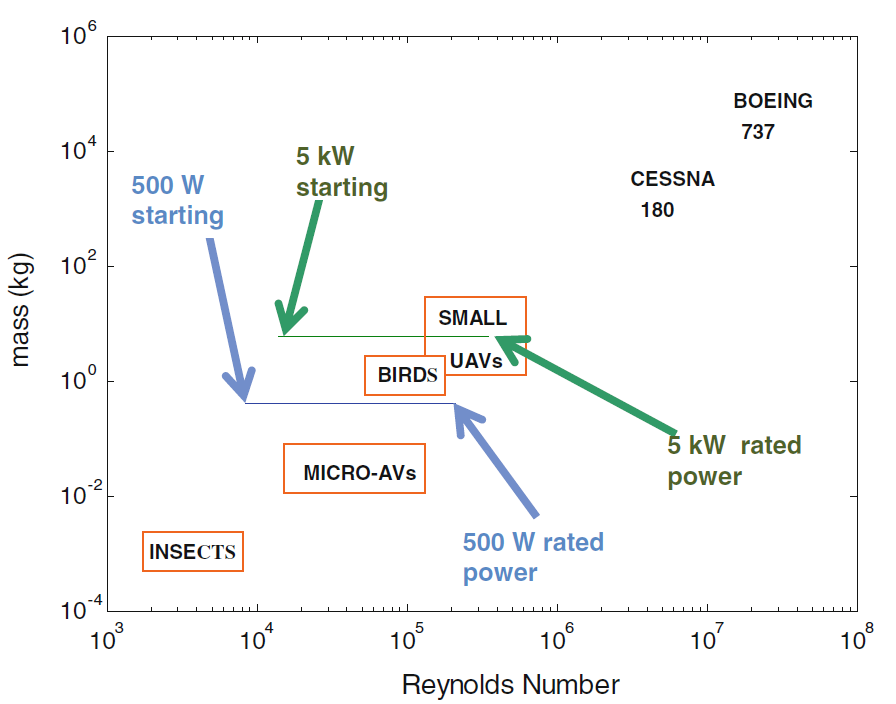
\includegraphics[width=0.6\linewidth]{Images/Low_RE_Number}
	\caption[Reynolds number ranges]{Reynolds number ranges for small wind turbines and other aerodynamic bodies. \\
		Obtained from \cite{Wood}.}
	\label{fig:LowReNumber}
\end{figure}

\FloatBarrier

The airfoils will be studied using XFOIL sofware with XFLR5 graphical user interface. As it uses an inviscid linear-vorticity panel method with a Karman-Tsien compressibility correction, this software shows reliable results for low Re flows. Note that it was initially intended for the calculation of model sailplanes. The following constant parameters need to be defined to set up the simulation \cite{fuentes2016airfoil}: 

\begin{enumerate}
	\item \textbf{Mach number}: As XFOIL considers incompressible flow (M=0) any value below 0.3, this value is initially defined as $M=0$.
	
	\item \textbf{Boundary layer transition}: It is assumed that the laminar to turbulent transition will occur due to the roughness of the blades. The XFOIL documentation is followed, and a value of Ncrit = 1 is set. \cite{XFOIL} 
		 
	\item \textbf{Reynolds number}: Although reliability can be expected from XFOIL results, the error increases at significant low Reynolds. The following Reynolds will be studied: $Re=2\cdot10^5$, $Re=1.6\cdot10^5$, $Re=1.2\cdot10^5$, $Re=8\cdot10^4$, and $Re=4\cdot10^4$.
\end{enumerate}



%It is known that lift and drag coefficients depend on the Reynolds number. Although computational analysis is very used for airfoil study, there are authors that state these results can not be completely trusted at low Re \cite{Wood}. There is also low accurate experimental data available for these cases ($Re<10^5$) due to the small forces involved. In order to reduce uncertainties and ensure veracity of the data used, this design will be limited to a little amount of well-studied airfoils designed specifically for small wind turbines. 

\subsubsection{Airfoils studied}

The following table summarizes the airfoils that will be tested and studied. The airfoil coordinates and the values presented below has been obtained from \textit{airfoiltools.com} \cite{Airfoiltools}, a useful website that uses UIUC's airfoil database \cite{UIUC}. All the airfoils studied have been designed looking for a good performance in low Reynolds number operation. Some of them are specifically designed for small wind turbines: SG series (Selig-Giguere) and S833/4/5 airfoils designed by NREL are probably the first aerofoils designed for this purpose \cite{Wood}. The other models have been selected by looking into low Reynolds airfoils studies \cite{fuentes2016airfoil} \cite{shah2012low}.  

\begin{center}

	\rowcolors{4}{}{lightgray}
	\begin{longtable}{C{1cm}|C{2cm}|C{2.2cm}C{1.5cm}|C{2.2cm}C{1.5cm}}
	\caption[Airfoils selected to be studied.]{Airfoils selected to be studied. All values are indicated in chord percentage.}	\label{tab:Airfoils_Studied}  \\ 
	Code &	Airfoil & Maximum thickness [\%]& Position [\%]   & Maximum camber [\%]& Position  [\%]                                \\ \hline \endhead
	1&	SG6040  & 16.0           & 35.3                  & 2.3       & 60.5                \\
	2&	SG6041  & 10.0           & 34.9                 & 1.5       & 49.7                \\
	3&	SG6042  & 10.0           & 33.5                 & 3.3       & 51.5                \\
	4&	SG6043  & 10.0          & 32.1                  & 5.1       & 53.3               \\
	5&	S833    & 18.0           & 36.3                  & 2.5       & 78.8                  \\
	6&	S834    & 15.0           & 39.5                  & 1.6       & 60.0                    \\
	7&	S835    & 21.0           & 30.5                  & 2.4       & 78.0                   \\
	8&	S1210   &   12.0            &     21.4       &   6.7          &    51.1           \\
	9&	S1223   &   12.1          &     19.8          &     8.1        &  49.9               \\
	10&	S6063   &     7.0        &       29.4           &     1.3        &   43.8          \\
	11&	S9037   &     9.0        &    28.5              &   3.3    &       42.4          \\
	12&	S3010   &     10.3	     &  	25        &    2.3         &       43.3            \\
	13&	SD8000  &       8.9     &     29.4        &    1.5       &       54               \\
	14&	BW3     &      5.0           &      7.4        &    5.7         &    45.4             \\
	15&	E387    &      9.1        &      31.1       &     3.2        &    44.8           \\
	16&	E374    &    10.9         &    34.3         &    2.0       & 38.9             \\
	17&	E62     &     5.6            &       26.2       &     5.0        &      49.3         \\
	18&	RG15    &      8.9           &      30.2            &    1.8         &  39.7		
	\end{longtable}

\end{center}

\FloatBarrier

The following parameters will be analyzed for each airfoil:

%%JUSTIFICAR CADA PARÀMETRE

\begin{enumerate}
	\item Maximum efficiency $E$: 
	\item $\Delta \alpha=\alpha_{s}-\alpha_{opt}$: 
	\item $\dfrac{d\alpha_{opt}}{dRe}$:
	\item $\dfrac{dE}{dRe}$:
	\item $\dfrac{dE}{d \alpha} (\alpha=\alpha_{opt})$
	\item Thickness $t/c$:
	\item $Cl_{opt}$: 
	
\end{enumerate}







\subsection{Blades design}
	
	
\end{document}